% !TEX root = ../Bachelorthesis.tex
%
%************************************************
% Einführung
%************************************************
\chapter{Einführung}
\label{sec:Einfuehrung}

Springer Nature ist ein weltweit führender Verlag für Forschungs-, Bildungs- und Fachliteratur mit einer breiten Palette an angesehenen und bekannten Medienmarken und zudem der weltweit größte Verlag für Wissenschaftsbücher. Für das Unternehmen Springer Nature ist es darum wichtig, auf seinen Web-Applikationen eine Suche anbieten zu können, die Suchintentionen erkennt und möglichst schnell zum gesuchten Content leitet. Die Suche wird vor allem als Hilfsmittel zur Navigation und zum Finden von Literatur und Dienstleistungen genutzt. Durch die vielen von Springer Nature publizierten\footnote{Unter publizieren wird in dieser Arbeit die Veröffentlichung auf der Springermedizin-Applikation bezeichnet} Zeitschriften und Querverweise in Artikeln, wird sie aber auch oft zur Suche nach Issues\footnote{Nummer der Zeitschriftenausgabe, in der sich der Artikel befindet.} und Artikeln verwendet sowie als Hilfestellung um Diagnosen zu Krankheitsbilder stellen zu können.
\\
\\
Springer Nature sammelt viele User-Tracking-Daten und dadurch viel Wissen über das Verhalten der User\footnote{Als User werden die Nutzer der Springer Nature Suche bezeichnet} bei der Nutzung ihrer Suche, lässt dieses Wissen jedoch bisher noch nicht in ihre Suche einfließen. In dieser Arbeit wollen wir untersuchen, ob mithilfe dieses Wissens, die Suche optimiert werden kann.

% Aufbau der Suche bei Springer Nature
%------------------------------------------------

\section{Aufbau der Suche bei Springer Nature}
\label{sec:Einfuehrung:AufbauSucheBeiSpringerNature}

\subsubsection{White Label Applikation mit Solr-Suche}
\label{sec:Einfuehrung:AufbauSucheBeiSpringerNature:WhiteLabelApplikationSolr-Suche}

Damit die verschiedenen Verlage und Zeitschriften der Verlagsgruppe Springer Nature ihre Produkte und Dienstleistungen online anbieten können nutzt Springer Nature eine eigens entwickelte White Label Applikation\footnote{Eine White Label Applikation ist eine wiederverwendbare und agil erweiterbare Applikation}. Die White Label Applikation verwendet \textit{Apache Solr}~(im Folgenden \glqq Solr\grqq{} genannt, siehe \cite{solr}) als Suchplattform. Die Solr dient hierbei als eine der Schnittstellen zwischen dem Content-Pool von Springer Nature und der White Label Applikation. Bei den vom Content-Pool gelieferten Inhalten, handelt es sich um von Springer Nature Verlag publizierte Zeitschriften, Artikel, Bücher und redaktionelle Inhalte.

\subsubsection{User-Tracking mit Webtrekk}
\label{sec:Einfuehrung:AufbauSucheBeiSpringerNature:Webtrekk}

Um das Verhalten der User auf ihren Web-Applikationen zu tracken verwendet Springer Nature das Analysetool Webtrekk~(siehe \cite{webtrekk}). Die daraus resultierenden Berichte bieten unter anderem die Möglichkeit, \textit{Suchquery-Logs}\footnote{Protokoll über alle ausgeführten Suchanfragen auf der Applikation} und \textit{Click-Trough-Rates} (CTR)\footnote{Kennzahl um die Anzahl der Klicks auf Links im Verhältnis zu den gesamten Impressionen darzustellen} der User auszuwerten.

\pagebreak

\subsubsection{Architektur}
\label{sec:Einfuehrung:AufbauSucheBeiSpringerNature:Architektur}

In Abb. \ref{fig:SucheSpringerNature} ist die Suche nochmals grafisch aufbereitet:

\begin{figure}[H]
\centering
\vspace{-1.25em}
\caption[Aufbau der Suche bei Springer Nature]{Aufbau der Suche bei Springer Nature}
\vspace{.5em}
\label{fig:SucheSpringerNature}
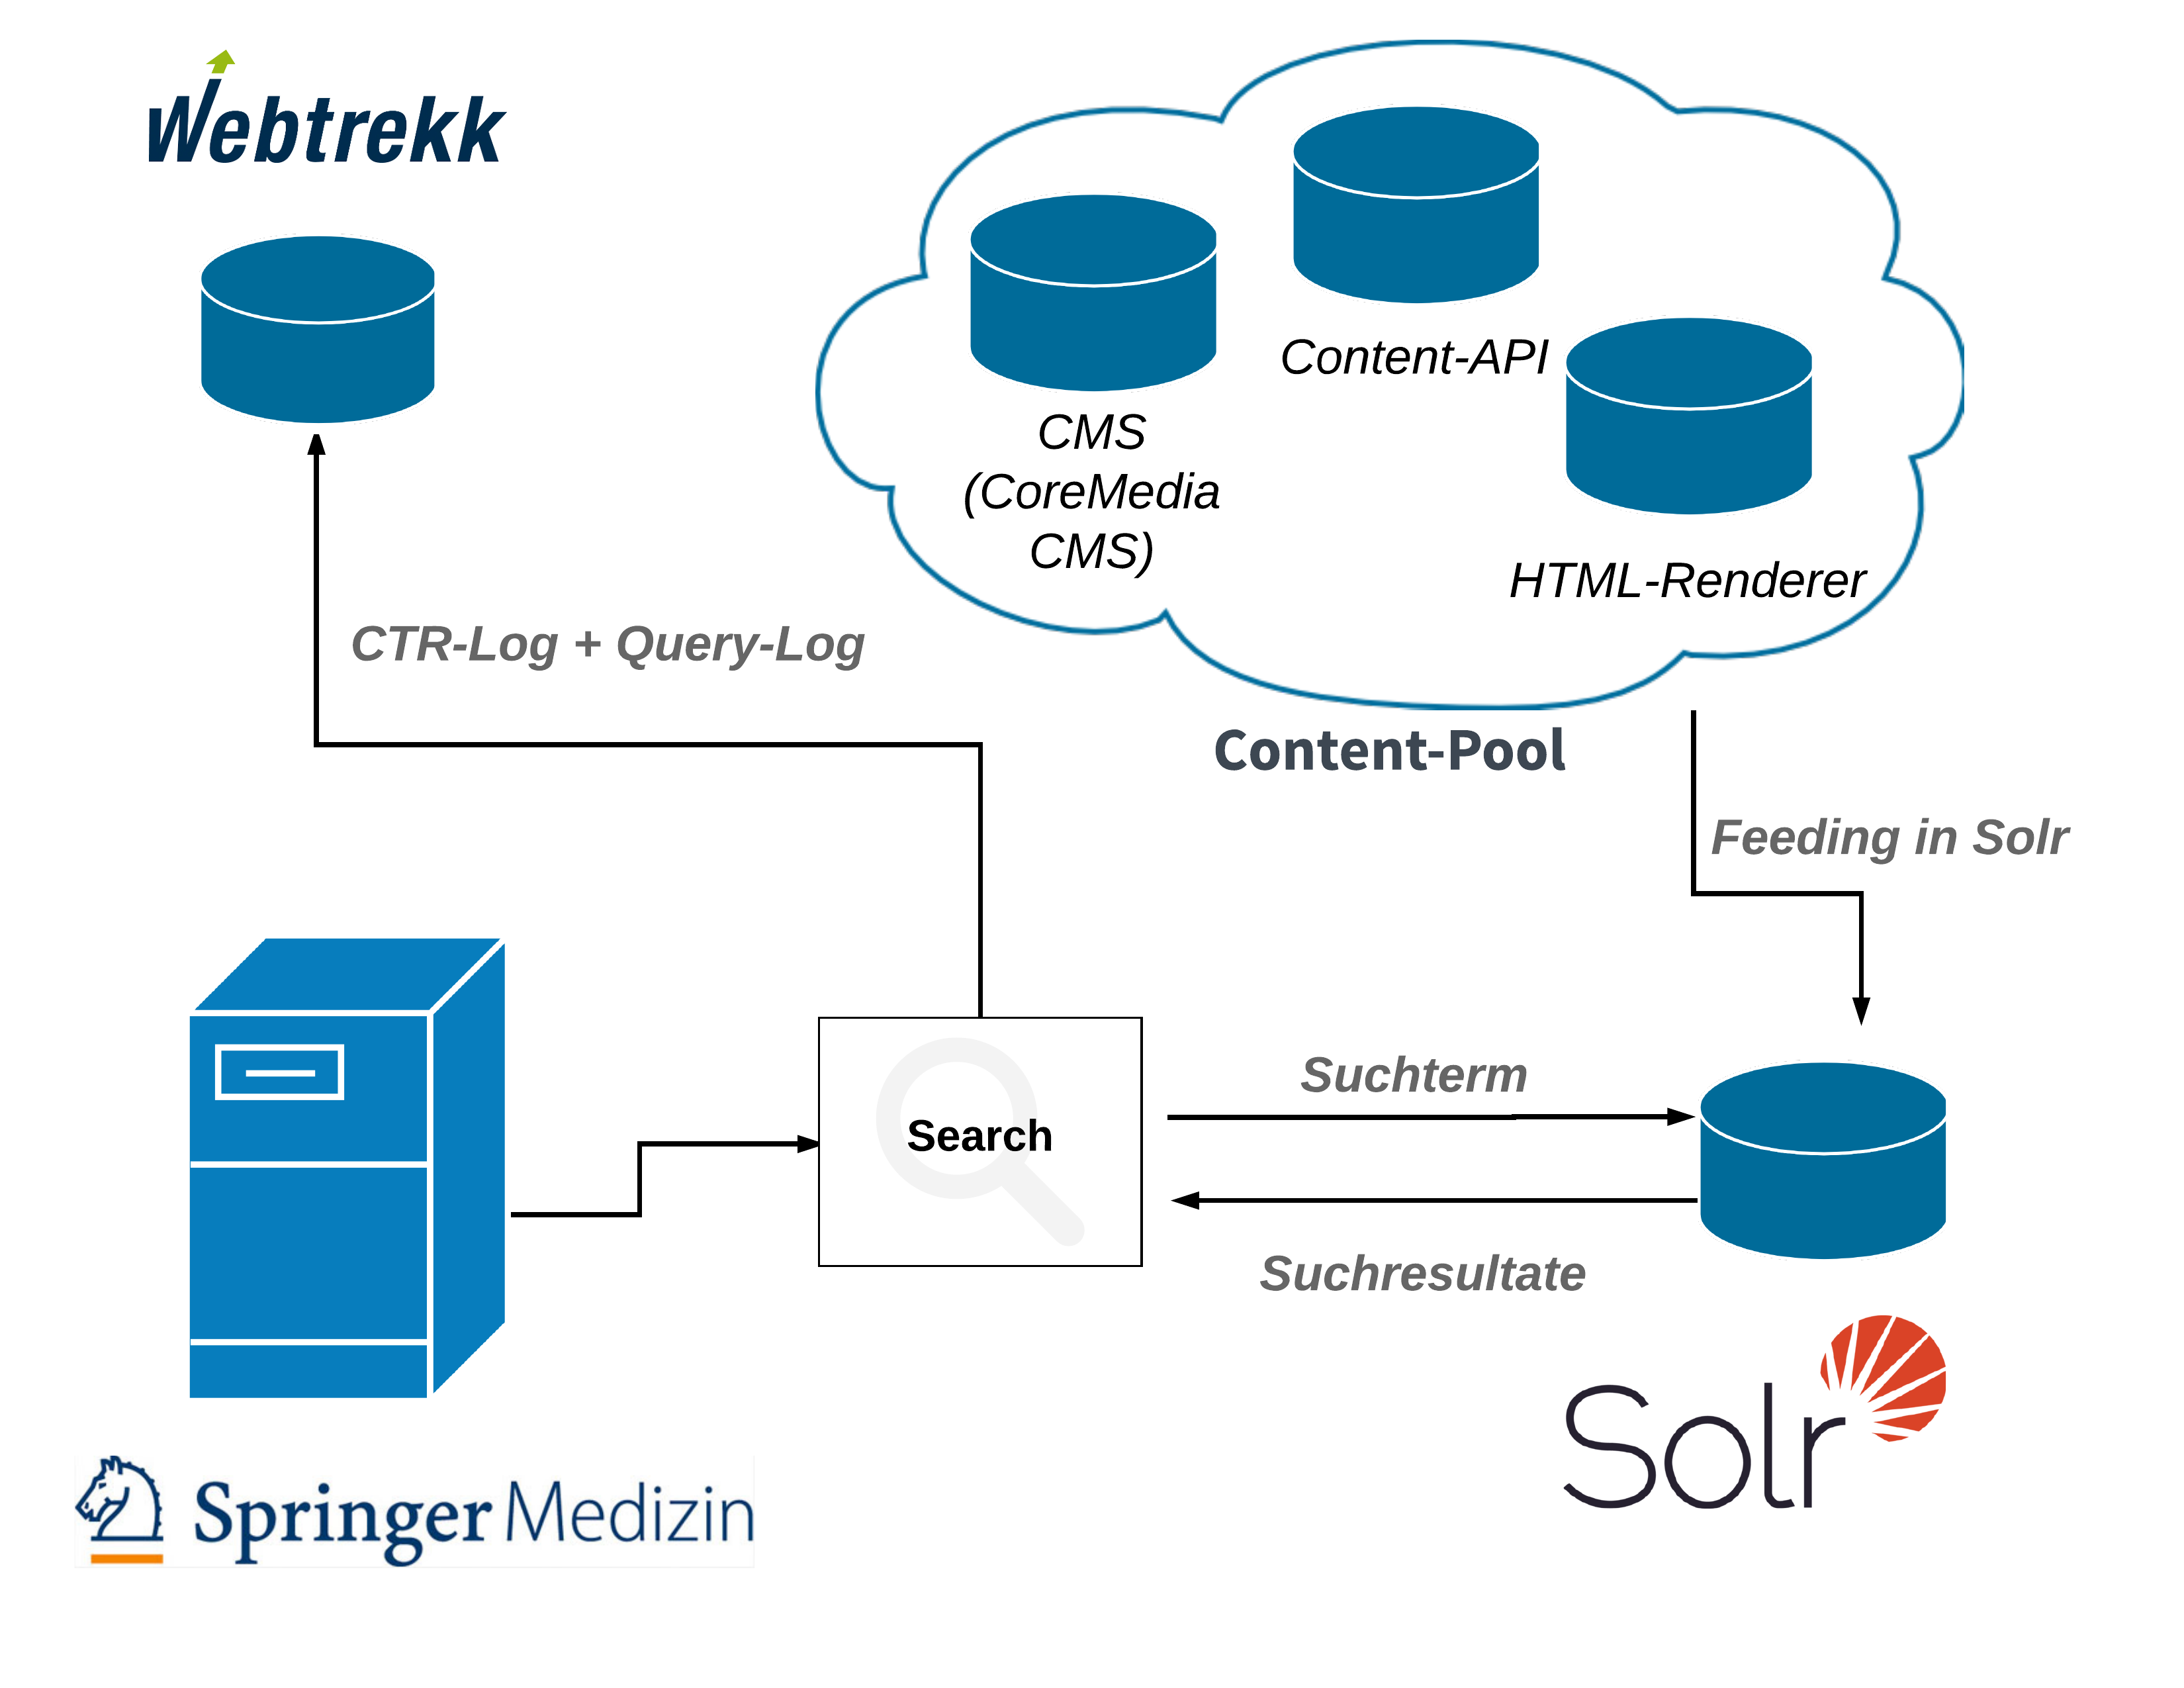
\includegraphics[width=0.5\linewidth]{gfx/AufbauSucheSpringerNature}
\vspace{-2em}
\end{figure}

% Problemstellung: Keine Userrelevanz in der Suche
%------------------------------------------------

\section{Problemstellung: Keine Userrelevanz in der Suche}
\label{sec:Einfuehrung:Problemstellung}

Zu den Stakeholder\footnote{Bezeichnet Springer Nature interne Kunden, die ein Interesse am Ergebnis der White Label Applikation haben} der in Kapitel \ref{sec:Einfuehrung:AufbauSucheBeiSpringerNature:WhiteLabelApplikationSolr-Suche} angesprochenen White Label Applikation gehört \textit{Springermedizin}~(siehe \cite{SMED}). Springermedizin betreibt ein Fortbildungs- und Informationsportal für Ärzte.

\subsubsection{Userrelevante Dokumente werden nicht gefunden}
\label{sec:Einfuehrung:Problemstellung:Userrelevanz}

Die User von Springermedizin suchen oft mit einschlägig, fundierten Fachbegriffen nach den neuesten und relevantesten Zeitschriften, Bücher oder Publikationen. Die zeitlich aktuellsten Suchtreffer zu finden ist für Springermedizin kein Problem. Die für den User \textit{relevantesten} jedoch schon.

\subsubsection{Der Springer Nature Stakeholder: Springermedizin setzt auf Webtrekk}
\label{sec:Einfuehrung:Problemstellung:Springermedizin}

Mithilfe von Webanalysten und Webtrekk versucht Springermedizin das Marketing seines Webauftrittes zu verbessern und ist sehr interessiert an neuen Ansätzen, um die gesammelten Tracking-Daten besser einzusetzen. In dieser Arbeit wird darum der Fokus auf die Verwendung von Tracking-Daten in der Suche von Springermedizin gesetzt. 
 
\subsubsection{Der fast gläserne User}
\label{sec:Einfuehrung:Problemstellung:Glaeserne-User}

Springermedizin sammelt Tracking-Daten über jegliche Aktivitäten auf deren Applikationen und investiert Zeit und Geld in die Individualisierung\footnote{Mit Individualisierung wird die Speicherung eigener Parameter bezeichnet} der Analysedaten auf Webtrekk. Mittlerweile sind knapp 30 Custom-Parameter\footnote{Individuell erzeugte Parameter für Berichte und Analysen} auf Webtrekk angelegt um genau die Daten zu tracken, die zur Analyse des Verhaltens der User auf ihrer Applikationen relevant sind. Dadurch entsteht ein fast \glqq gläsernen User\grqq{}. Dieses Wissen könnte zum Vorteil des Users eingesetzt werden, indem es in der Suche verwendet wird.

\pagebreak
% Ziel der Arbeit
%------------------------------------------------
\section{Ziel der Arbeit}
\label{sec:Einfuehrung:ZielArbeit}

\subsection{Suchoptimierung durch Click-Trough-Daten}
\label{sec:Einfuehrung:ZielArbeit:Suchoptimierung}

In dieser Arbeit werden wir untersuchen, ob mithilfe der von Springermedizin gesammelten Click-Trough-Daten\footnote{Mit Click-Trough-Daten bezeichnen wir alle Tracking-Daten, welche während der Interaktion zwischen User und Suche protokolliert werden} dessen Suche verbessert werden kann. Konkret wollen wir dies anhand eines Algorithmus basierend auf dem Klick-Modell\footnote{Als Klick-Modell wird ein Modell zur Berechnung des Userfeedbacks bzw. der Userrelevanz mithilfe von Click-Trough-Daten bezeichnet} \textit{Position-Based Modell}~(PBM, siehe \cite{pbm}) untersuchen.

\subsubsection{Annahmen}
\label{sec:Einfuehrung:ZielArbeit:Suchoptimierung:Annahmen}

Wir gehen dabei von folgenden Annahmen aus. Relevante Dokumente sind wichtiger als nicht relevante Dokumente. Eine Suchergebnis ist dann gut, wenn die relevanten Ergebnisse in der verwendeten Hierarchie vor den nicht relevanten Ergebnisse auftauchen. 

\subsubsection{Anwendung auf das Springermedizin-Umfeld}
\label{sec:Einfuehrung:ZielArbeit:Suchoptimierung:AnwendungSpringermedizin-Umfeld}

Wir werden versuchen, die Click-Trough-Rates der Suchresultate mithilfe des oben angesprochenen Algorithmus zu berechnen und mit diesen ein \textit{Reranking}\footnote{Mit Reranking bezeichnen wie die Umsortierung einer Liste von Suchresultaten} der Suchresultate auf das Springermedizin-Umfeld abzubilden. Die Herausforderung wird hierbei die Adaptierung des Lösungsansatzes auf das Springermedizin-Umfeld sein. Im Idealfall widerspiegeln die gesammelten Click-Trough-Daten der Userrelevanz der einzelnen Dokumente\footnote{Als Dokumente werden die einzelnen Suchresultate bezeichnet}.

\subsection{Abbildung auf das Springermedizin-Umfeld}
\label{sec:Einfuehrung:ZielArbeit:AbbildungSpringermedizinUmfeld}

\subsubsection{Potential von Userrelevanzen in der Suchoptimierung analysieren}
\label{sec:Einfuehrung:ZielArbeit:Potential}

Die Analyse von User-Tracking-Daten bietet viel Potential bezogen auf Userrelevanzen. Sind anhand des hier umgesetzten Lösungsansatzes Verbesserungen in der Qualität der Suche zu verzeichnen, möchte Springermedizin in Zukunft vermehrt User-Tracking-Daten in die Suche einfließen lassen. Diese Arbeit könnte dann als Fundament für weitere Lösungsansätze dienen.

\subsubsection{Bekanntes und wirkungsvolles Information Retrieval Verfahren}
\label{sec:Einfuehrung:ZielArbeit:AbbildungSpringermedizinUmfeld:InformationRetrievalVerfahren}

Suchoptimierung mittels Userrelevanz ist ein bekanntes und nicht triviales, aber relativ wirkungsvolles Information Retrieval Verfahren~(siehe \cite{IWUSBI}). Seit Mitte der 2000er Jahre wird mithilfe dieses Verfahrens versucht, Suchmaschinen zu verbessern. Aus dieser Zeit stammen auch die ersten Ansätze um mithilfe von Click-Trough-Daten die Userrelevanz der Suchergebnisse zu berechnen~(siehe \cite{Joachims}).

\subsubsection{Lösungsansatz basierend auf Click-Trough-Daten aus Webtrekk}
\label{sec:Einfuehrung:ZielArbeit:AbbildungSpringermedizinUmfeld:Loesungsansatz}

Springermedizin führt ein eigenes Tracking der User durch und verwendet auf Webtrekk selbst definierte Tracking-Parameter. Dadurch hängt die Wahl des in dieser Arbeit zu untersuchenden Lösungsansatzes und dessen Umsetzung stark von den durch Webtrekk gegebenen Analyse-Daten ab.

\subsubsection{Keine Gegenüberstellung mit anderen Lösungsansätzen}
\label{sec:Einfuehrung:ZielArbeit:AbbildungSpringermedizinUmfeld:NichtBehandeln}

Durch den vorgegebenen Zeitraum für die Erstellung dieser Bachelorarbeit bedingt, werden wir den Lösungsansatz so wählen, dass er mit den Gegebenheiten bei Springermedizin sinnvoll und in diesem Zeitrahmen realistisch implementiert werden kann. Wir werden daher in dieser Arbeit keine Gegenüberstellung mit anderen Lösungsansätzen machen. 

% Methodik
%------------------------------------------------

\section{Methodik}
\label{sec:Einfuehrung:Methodik}

Wie in Kapitel \ref{sec:Einfuehrung:ZielArbeit:Suchoptimierung} angesprochen, wollen wir das Klick-Verhalten der User in der Suche analysieren, um mithilfe der daraus berechenbaren Click-Trough-Rates, die Suchergebnisse zu verbessern. Dieses Klick-Verhalten können wir aus den Click-Trough-Daten lesen. 

\subsubsection{Suchterm semantisch aufschlüsseln}
\label{sec:Einfuehrung:Methodik:SuchtermSegmentierung}

Um mit den Click-Trough-Daten arbeiten zu können, müssen wir zunächst die relevanten Click-Trough-Daten herausfiltern. Dazu müssen wir die Click-Trough-Daten dem \textit{Suchterm}\footnote{Als Suchterm wird eine Suchanfrage bezeichnet} der Anfrage zuordnen können. Zu den Click-Trough-Daten wird immer der Suchterm gespeichert, mit dem dabei gesucht wurde. Das heißt wir können eine Relation zwischen dem Suchterm der Click-Trough-Daten und dem Suchterm unserer Anfrage herstellen.
\\
\\
Die Click-Trough-Daten müssen aber nicht mit dem vollständigen Suchterm in Relation stehen. Sie können auch nur mit einem Wort, einem Teil des Suchterms oder einem Synonym eines dieser Worte in Relation stehen. Wir müssen darum den Suchterm semantisch aufschlüsseln um alle relevanten Click-Trough-Daten filtern zu können. 

\subsubsection{Aufbereitung Click-Trough-Daten}
\label{sec:Einfuehrung:Methodik:Click-Trough-Daten}

Können wir alle relevanten Click-Trough-Daten zu einer Suchanfrage filtern, müssen lernen wie wir diese richtig aufbereiten, um die Click-Trough-Daten berechnen zu können.  Ein wichtiger Punkt bei der Aufbereitung der Click-Trough-Daten ist die Interpretation des Relevanzfeedbacks der einzelnen Click-Trough-Daten. Nicht jeder Klick ist gleich relevant zu interpretieren. Die Relevanz eines Klicks hängt davon ab, welche Aktionen der User während dem Suchvorgang vor und nach dem Klick durchgeführt hat. Wir müssen darum zuerst analysieren, welche Informationen wir zu den Click-Trough-Daten aus Webtrekk lesen können.  Reichen die Informationen für detailliertere Interpretationen nicht aus, müssen wir alle Click-Trough-Daten als gleich relevant lesen.

\subsubsection{Result-Reranking mittels PBM basiertem Algorithmus}
\label{sec:Einfuehrung:Methodik:Result-RerankingPBM}

Wissen wir, wie wir die Click-Trough-Daten aufbereiten, können wir diese zur Berechnung der Click-Trough-Rate eines Dokumentes und somit dessen Userrelevanz einsetzen. Für die Verwendung dieser Userrelevanz müssen wir festlegen wann und in welcher Art wir sie einsetzen. Wie bereits in Kapitel \ref{sec:Einfuehrung:ZielArbeit:Suchoptimierung:AnwendungSpringermedizin-Umfeld} erwähnt, werden wir uns in dieser Arbeit auf die \textit{Aufbereitung} der Suchresultate aus der Solr konzentrieren und dort einen \textit{Reranking-Algorithmus} einbauen. 
\\
\\
Der Reranking-Algorithmus basiert auf einem \textit{Klick-Modell}. Dieser verwendet die Click-Trough-Daten, um daraus die Click-Trough-Rate eines Dokumentes zu berechnen. Die Wahl des Klick-Modells hängt darum von den Click-Trough-Daten und den darin enthaltenen Informationen ab. In dieser Arbeit werden wir veranschaulichen, warum wir den Ansatz des Position-Based Modells~(siehe \cite{pbm}) gewählt haben und wie wir den Algorithmus umgesetzt haben.

\subsubsection{Vergessen der alten Daten}
\label{sec:Einfuehrung:Vergessen}

Das Position-Based Modell berechnet Wahrscheinlichkeiten, um die Click-Trough-Rate eines Dokumentes zu einer Suchanfrage festzustellen. Dem Algorithmus muss dazu das notwendige Wissen entweder zur Verfügung gestellt oder antrainiert werden. Wird dem Algorithmus das Wissen antrainiert, benötigt der Algorithmus eine Möglichkeit, neues Wissen zu Lernen und altes zu Vergessen. 
\\
\\
Mit Webtrekk haben wir eine Wissensbasis, die durch die Springermedizin-Applikation automatisch um neue Click-Trough-Daten ergänzt wird. Das heißt wir müssen uns nicht um eine Möglichkeit zum Lernen neuer Daten kümmern. Wir müssen uns aber überlegen, wie wir altes Wissen vergessen und wie wir dem User neues Wissen präsentieren, damit dieser sich durch die Click-Trough-Rate-Berechnung nicht auf alten Dokumenten festfährt.

% Gliederung und Aufbau
%------------------------------------------------

\section{Gliederung und Aufbau}
\label{sec:Einfuehrung:GliederungAufbau}

\subsubsection{Der Lösungsansatz und deren Grundlagen}
\label{sec:Einfuehrung:GliederungAufbau:Loesungsansatz}

In diesem Kapitel wurde der zu untersuchenden Lösungsansatz vorgestellt. Dabei sind wir auf die Hintergründe dieser Arbeit und die Vorgehensweise eingegangen. Im zweiten Kapitel~(Grundlagen) folgt die Theorie des beschriebenen Lösungsansatzes. Hier werden wir uns auf die fachlichen Grundlagen konzentrieren. 

\subsubsection{Umsetzung des Lösungsansatzes}
\label{sec:Einfuehrung:GliederungAufbau:Umsetzung}

In Kapitel \ref{sec:Reranking}~(Reranking mittels Click-Trough-Rate Ergebnis) werden wir die in Kapitel \ref{sec:Einfuehrung:Methodik} angesprochene Methodik verfeinern und detailliert die Vorgehensweise bei der Umsetzung diskutieren. Die Umsetzung selbst folgt dann in Kapitel \ref{sec:Implementierung}~(Implementierung).

\subsubsection{Erkenntnisse verarbeiten}
\label{sec:Einfuehrung:GliederungAufbau:Erkenntnisse}

Um zu prüfen ob der umgesetzte Lösungsansatz die erhofften Verbesserungen erzielt, werden wir diesen in Kapitel \ref{sec:Evaluation}~(Evaluation und Auswertung) in einer Evaluation mit der bisherigen Springermedizin-Suche vergleichen. Aufgrund der resultierenden Erkenntnisse werden wir in Kapitel \ref{sec:ZusammenfassungAusblick}~(Zusammenfassung und Ausblick) ein Fazit ziehen können und einen Ausblick auf mögliche zukünftige Arbeiten geben.